\documentclass[11pt]{article}

%Don't change any thing before \begin{document}
%They are not useful for now, but later when you try to add figures
%these might be useful. In fact if you use sth fancy, you might need
%to add more packages, or macros.
\usepackage{amssymb,amsmath}
\usepackage{times,psfrag,epsf,epsfig,graphics,graphicx}
\usepackage{algorithm}
\usepackage{algorithmic}

\begin{document}
\date{}

\title{CSCI 246: Assignment~4~(5 points)}

\author{William Jardee}

\maketitle
\section*{Problem 1.}

\noindent
Use the test for primality to determine whether the following numbers are
prime or not; if not, list one factor greater than one.

{\bf Test for Primality:} ~~ Given an integer $n>1$, to test whether $n$ is
prime check to see if it is divisible by a prime number less than or equal to
$\sqrt{n}$. If it is not divisible by any of these numbers, then it is prime.
\newline

I wrote a quick script in Python to do the calculations for me:\\
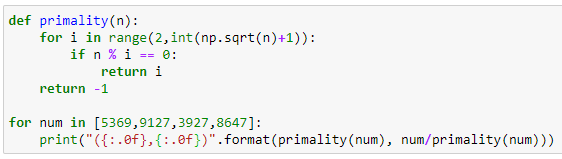
\includegraphics[width = \linewidth]{Homework/pic_1.PNG}\\

\noindent
(1.1) 5,369.\\
This number is not prime, the first factor greater than 1 is 7.\\

\noindent
(1.2) 9,127.\\
This number is prime.\\

\noindent
(1.3) 3,927.\\
This number is not prime, the first factor greater than 1 is 3.\\

\noindent
(1.4) 8,647.\\
This number is prime.\\

\newpage


\section*{Problem 2.}

\noindent
Compute the following, assume that $n>4$.
$$\frac{(n-1)!}{(n-5)!}$$
\newline 
\[\frac{(n-5)!(n-4)(n-3)(n-2)(n-1)}{(n-5)!} = (n-1)(n-2)(n-3)(n-4)\]

\newpage

\section*{Problem 3.}

Prove the following statement by mathematical induction.

For every integer $n\geq 0$, $\sum\limits_{i=1}^{n+1}i\cdot 2^i=n\cdot 2^{n+2}+2$.
\newline

{\bf Proof by Induction:}\\

Base Case:\\
Let $n=0$. Then $\sum\limits_{i=1}^{n+1} i\cdot 2^i = 2$. The right side is $n\cdot 2^{n+2}+2 = 2$. So the base case of $n=0$ holds.\\

Inductive step:\\
Let us assume that the case of $k_n$ holds, now we must show that it holds for $k_{n+1}$.\\
\[\sum_{i=1}^{n+2} i \cdot 2^i = \Big(\sum_{i=1}^{n+1} i \cdot 2^i\Big) + (n+2)\cdot 2^{n+2} = n\cdot 2^{n+2} +2 + (n+2)\cdot 2^{n+2}\]
\[= (2n+2)\cdot 2^{n+2} +2 = 2\cdot(n+1)n^{n+2} + 2 = (n+1)n^{n+3} + 2 = (n+1)2^{(n+1)+2} + 2\]
\\
So if any $k_n$ works, then $k_{n+1}$ also works. Since our base case was $n=0$, we can say that the identity $\sum\limits_{i=}^{n+1} i\cdot 2^i = 2^i=n\cdot 2^{n+2}+2$ holds for any $n\geq 0$.
\begin{flushright}$\blacksquare$\end{flushright}




\newpage

\noindent
\section*{Problem 4.}

Use the formula for the sum of a geometric sequence to write the following sum in a closed form.
\newline

$8+8^2+8^3+\cdots 8^k$, where $k\geq 1$ is an integer.
\newline

Using the equation for a geometric sums: $S_n = \frac{a(r^n -1)}{r-1}$ where the terms follow the rule $a_n = ar^{n-1}$:
\[S_n = \frac{8\cdot (8^n -1)}{8-1} \rightarrow S_n =\frac{8}{7}(8^k -1)\]

\newpage


\section*{Problem 5.}

Prove the following statement by mathematical induction.
\newline

For every integer $n\geq 0$, $2^n<(n+2)!$.
\newline

{\bf Proof by Induction}\\

Base Case:\\
Let $n=0$, then $2^0 = 1 < 2 = (n+2)!$. So the $n=0$ case holds.\\

Inductive Step:\\
Let us assume that the $k_n$ case works, so let us prove the $k_{n+1}$ case also works.\\
Left Side: \quad  $2^{n+1} = 2\cdot 2^n$\\
Right Side: \quad $(n+1+2)! = (n+3)(n+2)!$\\

Our base case outlined that $n=0$, so every step greater than that will be positive. So: $n\geq 0 \rightarrow n+3 \geq 2$. The following logic then follows:
\begin{center}
    $2^n < (n+2)!$ \quad {\it $k_n$ step}
\end{center}
\[2\cdot 2^n < 2 \cdot (n+2)! < (n+3)(n+2)! \rightarrow 2^{n+1} < ((n+1)+2)!\]

So, our base case held and we have shown that, through induction, any steps larger than $n=0$ will also hold. So, the following identity is true:
\[ n\geq 0 \rightarrow 2^n<(n+2)!\]
\begin{flushright}$\blacksquare$\end{flushright}

\end{document}
